
\section{Preliminaries}

\subsection{Submanifolds}

Often in mathematics there is an obvious notion of a ``subobject'': given a structure on a set there is a simple way to restrict it to a subset, such that the subset can be said to have the same structure.
For example, the structure on a group is the identity, inversion, and multiplication; if there is a subset containing the identity and which is preserved under inversion and multiplication, then we have a subgroup.
Or for a topological space $X$, any subset $A$ has a topology given by intersection of open sets of $X$ with $A$.
The structures on the subset can often be characterised by the fact that they make the inclusion map $A \hookrightarrow X$ a structure preserving map (group homomorphism and continuous map respectively for the two examples).

In the case of manifolds however the definition of a submanifold is not as trivial and there are several notions that have strong claims for the title.
To complicate matters, the notion that is the most widely taught and used (embedded submanifold) is not the one that is most appropriate for Lie group theory (immersed submanifold).
Further, the two perspectives of the first paragraph, restriction and inclusion, each have their advantages.
It is perhaps more intuitive to work directly with a subset, but a manifold structure is an atlas, and it unpleasant to consider different atlases on the same subset.
The alternative is to work with inclusion maps.
Then different manifold structures of the subset are realised as inclusion maps from different manifolds with the same image.
% Our two main sources for this section are Sharpe and Warner.

\begin{definition}\textup{\cite[Def~1.27, Rem~1.33]{Warner1983},\cite[Defs~1.1.36,~1.1.40,~1.2.10,~1.2.21]{Sharpe1997}} \\
Let $\phi : N \to M$ be a smooth map of manifolds.
\begin{enumerate}
\item 
$\phi$ is called an \emph{immersion} if $d\phi_p : T_pN \to T_{\phi(p)}M$ is injective at every point $p \in N$.
The pair $(N,\phi)$ is called an \emph{immersed manifold} in $M$.
% \item 
% $\phi$ is called a submersion if $d\phi_p : T_pN \to T_{\phi(p)}M$ is surjective at every point $p \in N$.
\item
If $\phi$ is an injective immersion then the pair is called an \emph{immersed submanifold}.
\item 
Two immersed submanifolds $(N_1,\phi_1)$ and $(N_2,\phi_2)$ are called \emph{equivalent} if there is a diffeomorphism $\varphi : N_1 \to N_2$ such that $\phi_1 = \phi_2 \circ \varphi$.
\item
If an injective immersion $\phi$ has the property that for every smooth map $f: S \to M$ with $f[S] \subset \phi[N]$ the map $\phi^{-1} \circ f : S \to N$ is smooth, then we call $\phi$ a \emph{weak embedding} and the pair a \emph{weakly embedded submanifold}.
\item
If an immersion $\phi$ is a homeomorphism from $N$ to $\phi(N)$, the latter with the subspace topology of $M$, then we call it an \emph{embedding} and the pair is called an \emph{embedded submanifold}.
\item
A continuous function between Hausdorff spaces is called \emph{proper} if the preimage of a compact set is always a compact set.
A proper immersion submanifold is called a \emph{proper submanifold}.
\end{enumerate}
\end{definition}

This is a lot of terminology, but it harmonises the definitions in Sharpe and Warner, see below table.
It is in fact a strict hierarchy: each type of submanifold is a subtype of the previous.

\begin{table}[h]
\begin{tabular}{l|l|l}
 & Sharpe & Warner \\ \hline
immersed manifold & immersed manifold & \\
immersed submanifold & immersed submanifold & submanifold \\
weakly embedded submanifold &  &  \\
plaque submanifold & submanifold &  \\
embedded submanifold & regular submanifold & imbedding \\
proper submanifold & proper submanifold & proper submanifold \\
\end{tabular}
\end{table}

These definitions are given in terms of a smooth map into $M$.
So the question from the other perspective is whether the manifold structure of $N$ is determined or can be recovered solely from the image $\phi[N]$.
There are simple examples that show that not even the topology of $N$ is determined for an immersed submanifold: consider the subset $\{x^2 = y^2\} \subset \bbR^2$.
We can split this into a line and two rays in two ways.
Therefore immersed submanifolds must always be given with the immersion $\phi$.

Let us give a construction that can construct an atlas on a subset $N' \subset M$. TODO: Why is it $N'$?

\begin{definition}
\label{def:plaque submanifold}
\textup{\cite[Def~1.2.1,1.2.2,Thm~1.2.7]{Sharpe1997}}
Given a chart $\varphi: U \subset M \to \bbR^m$, the connected components of $N'\cap U$ are called plaques.
The intersection of open sets of $M$ with plaques gives $N'$ the \emph{submanifold topology}.
In general the submanifold topology is finer (has more open sets) than the subspace topology~\cite[Def~1.2.4]{Sharpe1997}.
% TODO: picture
For any plaque $W$, if $\varphi(W)$ lies in an $n$-dimensional affine subspace of $\bbR^m$ then we call this plaque flat and $\varphi|_W$ a plaque chart of $W$.
If there is a collection of charts $U_\alpha$ of $M$ that cover $\bar{N'}$ such that all components $U_\alpha\cap N'$ are flat plaques
we call $N'$ a plaque submanifold of $M$; the plaque charts constitute a smooth atlas.
\end{definition}

\begin{figure}[h]
\begin{center}
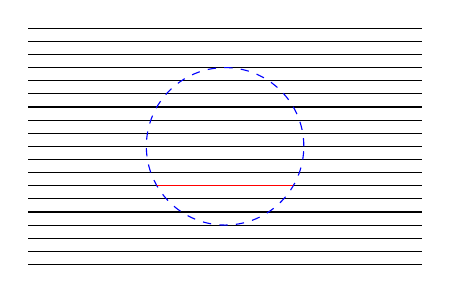
\begin{tikzpicture}[scale=0.5]
  % Draw 10 vertical lines closely bunched together
  \foreach \x in {0,1,2,...,18} {
    \draw (0,\x/3) -- (10,\x/3);
  }
  
  % Draw the circle
  \draw[dashed,blue] (5,3) circle (2);
  
  % Highlight one of the line segments in the circle
  \draw[red] (5-1.73,2) -- (5+1.73,2);
\end{tikzpicture}
\caption{$N'$ is the collection of black lines. The blue circle is an open subset of the plane, and the red segment is a plaque.}
\end{center}
\end{figure}

The plaque manifold structure on $N'$ makes the inclusion map into a weak embedding~\cite[Thm~1.2.7]{Sharpe1997}.
Unfortunately, the reverse is not true.
Consider $N$ as a countable collection of spheres and take $\phi : N \to \bbR^3$ to be the map that embeds the $k$th sphere as $\partial B(k^{-1}, 0.5(k+1)^{-2})$.
Overall one has a sequence of non-overlapping spheres decreasing in size with the origin as a limit point.
In particular any neighbourhood $U$ of the origin must contain a sphere as a connected component of $U \cap N'$.
But a sphere cannot be a flat plaque and therefore $N'$ is not a plaque submanifold.
It would be interesting to consider relaxations of the conditions to be a plaque submanifold.
% TODO: consider this.

The difference between plaque submanifold and embedded submanifold is that there is a covering of $N'$ by open sets of $M$ such that each chart has a single flat plaque.
This means that there can be no `strange' limits arising from the immersion.
For embedded submanifolds the subspace and submanifold topologies coincide~\cite[Prop~1.2.9]{Sharpe1997}.
The example of the dense wrapping of the line around a torus is the classic example of a plaque submanifold that is not embedded.

Finally, by \cite[Thm~1.2.11]{Sharpe1997} proper submanifolds are automatically embedded, so we have a strict hierarchy of conditions.
The standard example of an embedded submanifold that is not proper is $(0,1) \subset \bbR$.
We see that a sequence in $N$ may converge to a point of $M\setminus N$.

These constructions answer the question of how to endow a subset with a manifold structure.
There is the possibility however that there are different constructions.
Warner addresses these concerns with the following theorem: 
\begin{theorem}\label{thm:submanifolds}
\textup{\cite[Remark~1.33]{Warner1983}}
\begin{enumerate}
\item Let $M$ be a manifold and $A$ a subset of $M$. Fix a topology on $A$. Then there is at most one manifold structure on $A$ such that $(A,\iota)$ is an immersed submanifold of $M$, where $\iota$ is the inclusion map.
\item Again let $A$ be a subset of $M$. If $A$ with the subspace topology has a manifold structure such that $(A,\iota)$ is an immersed submanifold of $M$, then it is the unique topology on $A$ such that there exits a manifold structure for which $(A,\iota)$ is an immersed submanifold of $M$.
\end{enumerate}
\end{theorem}

We can strengthen Warner's theorem in light of the definition of plaque submanifold from Sharpe.
\begin{theorem}\label{thm:unique manifold structure}
Let $A$ be a subset of $M$. If $A$ with the submanifold topology of Definition~\ref{def:plaque submanifold} has a manifold structure such that $(A,\iota)$ is an immersed submanifold of $M$, then it is the unique topology on $A$ such that there exits a manifold structure for which $(A,\iota)$ is an immersed submanifold of $M$.
\end{theorem}
\begin{proof}
First we address the relationship between the manifold structure on $A$ and the plaque charts.
For any function $A \hookrightarrow M$ that is an immersion at $p$ the constant rank theorem gives us a plaque chart of $A$ at $p$.
Applying this to the inclusion $\iota$ and at every point we get that $A$ is a plaque submanifold.
By Part (a) of the previous theorem this is the unique manifold structure on $A$ with the submanifold topology (the manifold structure supposed in this theorem and the plaque charts belong to the same maximal atlas).

Now we move on to the statement in the theorem.
For clarity, let $B$ the manifold that has the same points as $A$ but a different topology and manifold structure, and let its inclusion be $j : B \hookrightarrow M$.
In terms of points, the composition $\iota^{-1} \circ j : B \to A$ is the identity map, so bijective.
We know that $(A,\iota)$ is a plaque submanifold, so it is a weak embedding.
Hence $\iota^{-1} \circ j$ is in fact a smooth map of manifolds.
Since both are immersions
At the corresponding step of the proof of Part (b) of the above theorem, Warner uses his Exercise~1.6
\end{proof}


\subsection{Distributions}

TODO: Revise this section, include proofs as necessary.

It is common in a course on manifolds to study vector fields and their integral curves.
The key local result is
\begin{theorem}[Picard-Lindelöff]
Let $F : J \times U \subset \bbR\times\bbR^n \to \bbR^n$ be a smooth time-dependent vector field. 
Assume $0 \in J$. 
Consider $u : \bbR \to U$ the system of ODEs $u'(t) = F(t,u(t))$.
For any $c \in U$ there exists a $\varepsilon > 0$ such that there is a unique solution smooth solution on $(-\varepsilon,\varepsilon)$ with $u(0) = c$.
Moreover, for any $p \in U$ there is an open neighbourhood $p \in V \subset U$, $\varepsilon > 0$ and smooth map $u : (-\varepsilon,\varepsilon) \times V \to U$ such that $u(\dot,c)$ is the unique solution with initial condition $c$.
\\\textup{\cite[Theorem~2.1.1]{Sharpe1997}}\cite[Theorem~1.2.1]{Ivey}
\end{theorem}

If one has a smooth vector field on a manifold, then this theorem provides for the existence of integral curves of the vector field in every coordinate chart, and uniqueness means that they can be patched together to give unique maximal integral curves through every point.

We will need a generalisation of this result that deals with multiple vector fields.
To motivate why this is geometrically interesting and not just generalisation for its own sake, consider a submanifold $N$ inside $M$.
At each point $p \in N$ we can consider the vector subspace $T_pN \subset T_pM$.
At least locally, we can describe these subspaces as the span of independent vector fields.
The natural question is the converse: given a set of independent vector fields on $M$, does there exist a submanifold $N$ whose tangent space is their span?
For a single vector field, the answer is affirmative, namely the integral curve.

\begin{definition}
An $r$-dimensional distribution $\mathcal{D}$ on $M$ is a choice of an $r$-dimensional subspace $\mathcal{D}_p$ of $T_p M$ at every point $p \in M$.
It is called smooth if every point has a neighbourhood and smooth vector fields $\{X_1, \dots, X_r \}$ that span the subspaces.
This is called a local basis for $\mathcal{D}$.
Equivalently, an $r$-dimensional distribution is an rank $r$ subbundle of $TM$.

A set of vector fields is called algebraically involutive if their Lie brackets are contained in their span.
Given two sets of vector fields with the same span, either one is algebraically involutive if and only if the other is.
Therefore algebraically involutive is a property that is defined for distributions.\\

A distribution is called integrable if every point has a coordinate neighbourhood in which the distribution is spanned by coordinate vector fields.
\\
A connected $r$-dimensional immersed submanifold $N$ is called an integral submanifold of $\mathcal{D}$ if at every point $T_pN = \mathcal{D}_p$.
\\\textup{\cite[2.2.1,.2.2.2,2.3.2]{Sharpe1997}}
\end{definition}

Consider the example of nested spheres centered at the origin in $\bbR^3\setminus\{0\}$. 
Their tangent planes define a $2$-distribution.
In a neighbourhood of any point, suitable polar coordinates show that it is smooth and integrable.
However there are not global vector fields spanning this distribution, due to the hairy ball theorem (every vector field on a sphere vanishes at least once).
By definition, any of the spheres is an integral manifold of this distribution.

The important example of a non-integrable distribution is given in $\bbR^3$ by the planes normal to the vector field $n(x,y,z)=(y,-x,1)$~\cite[Ex~2.3.1]{Sharpe1997}.
There can be no integral manifold containing the origin.
Suppose there were.
Because the tangent plane at the origin is the $xy$-plane, we know that there is a neighbourhood where is a graph over $x$ and $y$.
Now take a small loop in the integral manifold around the origin lying in this neighbourhood.
It's height is monotonic, it doesn't close up.
This is a contradiction.
A local basis at the origin is given by $X_1 = \partial_x - y \partial_z$, $X_2 = \partial_y + x\partial z$.
Observe that $[X_1,X_2] = 2\partial_z$, so that it is not algebraically involutive.


If a distribution is integrable, then every point has an integral submanifold through it, just by taking a coordinate plane in an appropriate chart.
And if there is an integral submanifold of the distribution at a point, the local basis of the distribution gives a vector field on it.
So then the Lie bracket is again tangent to the integral submanifold, showing that the vector fields are algebraically involutive at that point.
Hence algebraic involutive is a necessary condition to the existence of an integral submanifold.
The important theorem is Frobenius' theorem~\cite[2.4.1]{Sharpe1997}\cite[Thm~1.60]{Warner1983}, which states a distribution is integrable at a point if and only if it is algebraically involutive at that point.
The proof inductively applies the Picard-Lindelöff theorem.

In fact around each point $p$ there is a chart $(U,x)$ such that the flat plaques $V(q) = \{q' \in U | x_j(q') = x_j(q) \text{ for } m - r < j \leq m \}$ are integral submanifolds of the distribution, and any integrable submanifold contained in the chart is a subset of one of these.
In particular this is a plaque chart of any integral submanifold through $p$, hence it is a plaque submanifold.
Note that an integral submanifold may meet this chart several times, which explains why we don't have equality of sets above.
We can use uniqueness to unite integral submanifolds of a distribution into their maximal connected components.
Each of these is called a leaf and the collection of leaves is a foliation.

Perhaps let us revisit the example from the previous section of a weakly embedded submanifold that is not a plaque submanifold, the shrinking spheres.
There is no distribution on $\bbR^3$ with this as an integral submanifold. 
If we take a sequence of corresponding points on the spheres, $p_n = c_n + r_n \omega$ for $\omega \in \bbS^2$ for $c_n,r_n$ the centers and radii of the spheres, the limit is the origin. 
But all the tangent planes $T_{p_n}(\partial B(c_n,r_n))$ are parallel, so their limit is just any of them translated to the origin.
Taking several such sequences, we see that the distribution cannot be continuous at the origin.


% There is also a formulation of Frobenius' theorem in terms of differential forms.
% We can define the annihilator of a distribution as the algebraic ideal generated by the one-forms such that $\omega(v) = 0$ for all $v \in \mathcal{D}_p$.
% By this we mean all $C^\infty$-linear combinations and wedge products.
% Conversely, the kernel of an algebraic ideal of differential forms generated locally by $m-r$ independent one-forms is a distribution.
% The theorem then says that $\mathcal{D}$ is integrable if and only if the ideal contains all its exterior derivatives (it is a differential ideal).
% The proof comes down to the simple formula
% \[
% d\omega(X,Y) = X(\omega(Y)) - Y(\omega(X)) - \omega([X,Y]).
% \]

\subsection{Eigenvalues and Weights}

Eigenvalues and eigenvectors are ubiquitous in linear algebra.
If we are working over $\bbC$, then every linear endomorphism (linear map from a vector space $V$ to itself) has an eigenvalue (root of the characteristic polynomial) and every eigenvalue has an eigenvector $Av_\lambda = \lambda v_\lambda$.
If we can find a basis of eigenvectors, then with respect to this basis the linear operator is a diagonal matrix.
In general however, there may be fewer eigenvectors than the dimension of the vector space.
A standard result in linear algebra says that every matrix is conjugate to a matrix in Jordan normal form, unique up to reordering of the blocks.

Going further, we may ask what can be said of two linear endomorphisms $A,B$.
The key observation is to consider commuting operators.
If $A$ and $B$ commute then $B$ preserves the eigenspaces  eigenspaces of $A$:
\[
(A- \lambda I) (Bv) 
= B(A- \lambda I) v
= 0.
\]
Therefore $B$ restricts to an endomorphism on each of the eigenspaces of $A$.
Imposing different conditions on $A$ restricts the possible decompositions of $B$.
For example, if $A$ is diagonalizable (so $V$ decomposes as the direct sum of the eigenspaces of $A$) then on each eigenspace of $A$ we can choose a basis that puts $B$ into Jordan normal form.
Hence $A$ and $B$ can simultaneously conjugated to normal form.
Or if $A$ is diagonalizable and has no repeated eigenvalues, ie its eigenspaces are one dimensional, then these must also be eigenspaces of $B$.
Hence $A$ and $B$ are simultaneously diagonalizable.

This argument can be applied inductively to a finite set $\{A_1,\dots,A_k\}$ of pairwise commuting endomorphisms.
It also extends to a commuting family of operators $\mathcal{A} = \vspan\{A_1,\dots,A_k\}$, a linear subspace of $\End(V)$ such that all operators are pairwise commuting.
These are effectively equivalent, since a family is pairwise commuting if and only if a basis is pairwise commuting.
Likewise, $v$ is a simultaneous eigenvector for $\{A_1,\dots,A_k\}$ if and only if it is a simultaneous eigenvector for every operator of $\mathcal{A}$.
The eigenvalues are not completely independent:
\[
\lambda v
= Av 
= (a_1A_1 + \dots + a_kA_k)v
= a_1 \lambda_1 v + \dots + a_k \lambda_k v
= (a_1 \lambda_1 + \dots + a_k \lambda_k )v.
\]
We understand the eigenvalue of $v$ to be a linear function 
\[
\lambda : \mathcal{A} \to \mathbb{K}, 
\quad
\lambda(A) = a_1 \lambda_1 + \dots + a_k \lambda_k .
\]
Understood in this way, it is more common to call $\lambda$ a \emph{weight} of the commuting family $\mathcal{A}$, $v$ a \emph{weight vector}, and the set of vectors $v$ with $Av = \lambda(A)v$ the \emph{weight} space~\cite[Definition~A.14]{Hall2015}.

As an aside, the descriptor ``weight'' should probably replace ``eigen-'' even in the single operator case.
Consider an operator $A$ with a $2$-weight vector $v$ and a $3$-weight vector $w$.
Then of course $A(av+bw) = 2v + 3w$, which is a weighted sum.

We finish with an example.
Let $\mathcal{A}$ be the set of diagonal $n\times n$ matrices.
Then a basis for this family is $A_i = e_{ii}$, with $1$ at the $i$th position on the diagonal.
$e_i$ is a $1$-weight vector of $A_i$ while all vectors of $\vspan\{e_1,\dots,\hat{e}_i,\dots,e_n\}$ are $0$-weight (in the kernel).
These are all diagonal (in particular simultaneously diagonal) so there should be a basis of weight vectors.
Indeed, this is just the standard basis $\{e_1,\dots,e_n\}$.
The weight of $e_i$ is the linear form
\[
A = \operatorname{diag}(a_1,\dots,a_n) \mapsto a_i
\]
because $A e_i = a_i$.

